\documentclass{article}
\usepackage[utf8]{inputenc}
\usepackage[left=0.5in,right=0.5in,top=1cm,bottom=2cm]{geometry}
\usepackage{crop,graphicx,amsmath,array,color,amssymb,flushend,stfloats,amsthm,chngpage,times,fancyhdr,lipsum,lastpage}

%%%%%%%%%%%%   Header and Footer  %%%%%%%%%%%%%
\pagestyle{fancy}

\fancypagestyle{plain}{%
  \renewcommand{\headrulewidth}{0pt}%
  \fancyhf{}%
  \fancyfoot[R]{Page \bf\thepage\ \rm of \bf\pageref{LastPage}}%
}


%%%% Customise Titles and Headers: %%%%
\title{Be Right Back}
\author{Essay by Vishakha Kumaresan}
\date{\today}

\fancyhf{}
\fancyhead[L]{Vishakha}
\fancyhead[R]{19BCE2678}
\fancyfoot[R]{Page \bf\thepage\ \rm of \bf\pageref{LastPage}}


\begin{document}

%%%%%%%%%%%% Make Title and Format Lines %%%%%%%%%%%%
\maketitle											%
\vspace{-112px}										%
\noindent\rule{\linewidth}{1pt} \par				%
\vspace{100px}										%
\vspace{-20px}										%
\noindent\rule{\linewidth}{1pt} \par				%
\vspace{10px}										%
%%%%%%%%%%%%%%%%%%% Insert Logos %%%%%%%%%%%%%%%%%%%%	
\vspace{-85px}										%
\noindent											%
\begin{minipage}{0.5\textwidth}\begin{flushleft}	%
\hspace{20px}										%

\includegraphics[scale = 0.06]{vitlogo}		%
\end{flushleft}\end{minipage}						%
\begin{minipage}{0.5\textwidth}\begin{flushright}	%
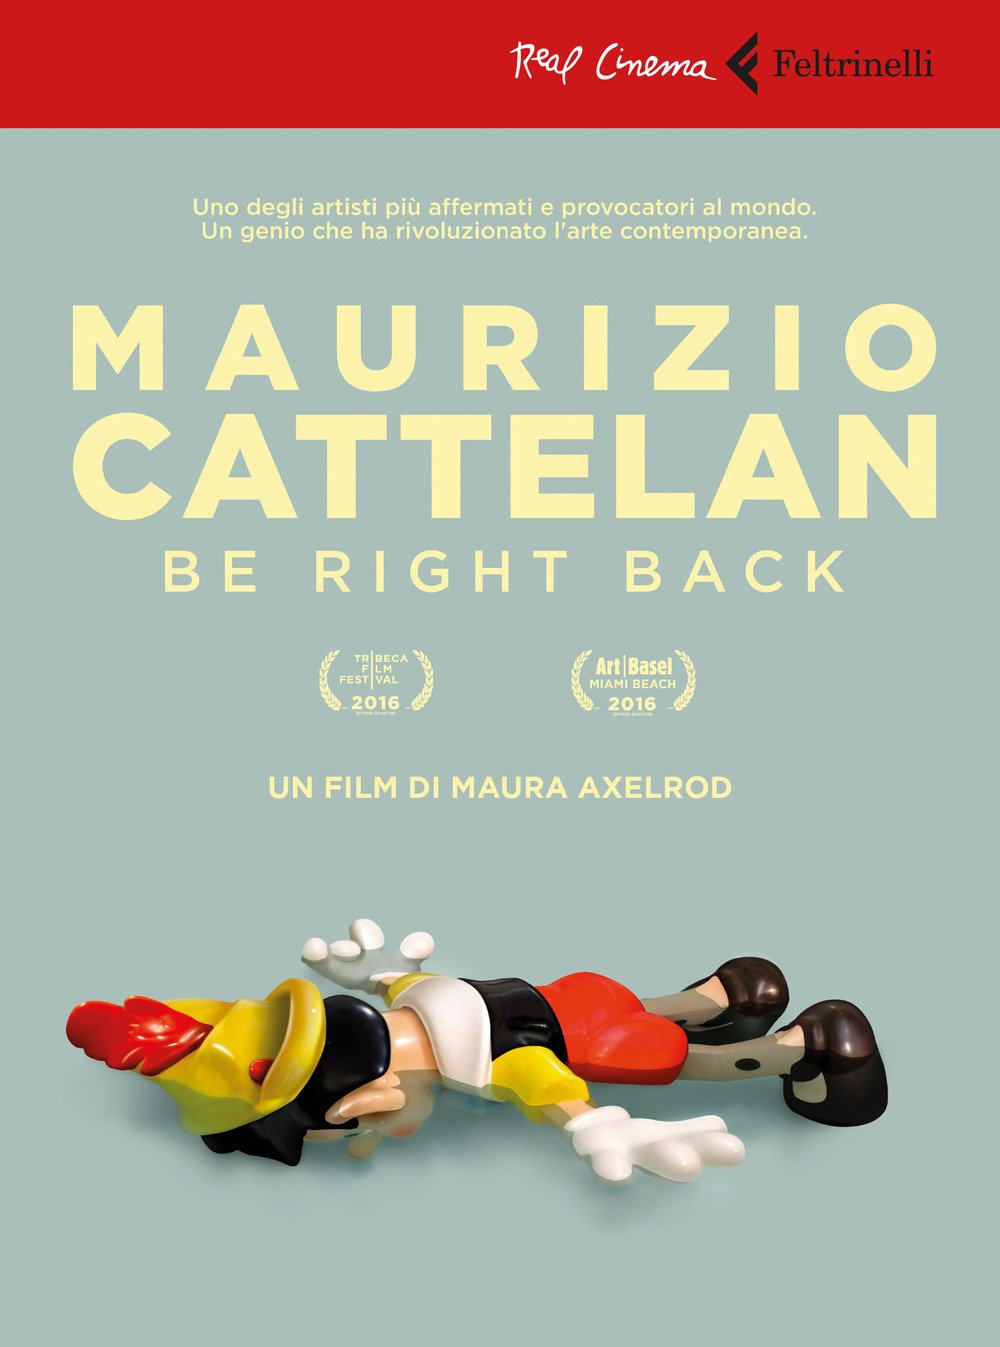
\includegraphics[scale = 0.05]{brb}		%
\hspace*{20px}										%
\end{flushright}\end{minipage}						%
\vspace{20px}										%
%%%%%%%%%%%%%%%% Headers and Footers %%%%%%%%%%%%%%%%

%Insert Body Text Here

I had the chance to watch Maurizio Cattelan: Be Right Back, a documentary directed by Maura Axelrod talking about the life of the infamous contemporary artist - Maurizio Cattelan. The documentary shows how he began his career, what kind of artist he was, and how he ended his career when he was at his peak. The documentary features some of his close friends, family and people he has worked along with.

His initial works described in the video came across as straight-up scams in my eyes as he blatantly changed the cover of a famous magazine, or faking a robbery of his work because he had nothing to put up. But this genius of him is what set him apart later on in his life.

From all the things he got away with including crimes like stealing and money scam, we can see how truly smart the Catellan is, all he had to do was put it to the right use.

His art portrayed what ‘out-of-the-box’ ideas truly meant. His ways drove a lot of controversy, be it any part of the world but nothing stopped him from bringing his ideas to life. The debatable piece of La Nona Ora, to conducting a fake biennale, Catellan had gotten himself the tag of a prankster in the field of art. 

The kind of art he made moving on were so bizarre and laughed upon but they had a deeper sense to them. For me personally, his works which involved hanging creatures/humans did disturb me a bit, but then I understand his intentions behind it. His works pulled crowd and fame along just by how unique they were and that’s what kept me glued to the documentary itself, I wanted to see what next weird thing could this man have thought of. His final presentation at Guggenheim which involved hanging his original pieces, showed his real character, his true surrender to art and as everyone who attended the event that night, I too was left in awe. 

The biggest thing which surprised me in the documentary was when it was revealed that the Maurizio Cattelan who was narrating his life all this while was not even the real Maurizio Cattelan, but it was an art curator named Massimiliano Gioni. Even though he retired early with probably years of ideas left within him, he did change the direction of contemporary art for the present world. 



\noindent\rule{\linewidth}{1pt} \par
1) Di dov'è Maurizio Cattelan?

A) Maurizio Cattelan è italiano di Padova

\noindent\rule{\linewidth}{1pt} \par
2) Massimiliano Gioni è spagnolo?

A) Massimiliano Gioni non è spagnolo, lui è italiano.

\noindent\rule{\linewidth}{1pt} \par
3) Among the titles of Cattelan's works, search at least three of them that are in Italian. What does each title mean if you translate it into English?

A)  3 of the many works by Maurizio Cattelan are as follows:

- Il Dito = The Finger

- La Nona Ora = The Ninth Hour

- La rivoluzione siamo noi = We are the revolution

\noindent\rule{\linewidth}{1pt} \par

LaTeX Link: https://github.com/Vishakha1909/BeRightBackItalian

\end{document}
